\section{Verification of Mobile Ad-hoc Protocols}\label{sec::wrebeca} 
%The computational model of Timed Rebeca makes it a faithful framework for modeling and analyzing network protocols based on asynchronous message passing, e.g., wireless protocols exploited in decentralized wireless networks.  
In decentralized wireless networks there is no pre-existing infrastructure, such as routers in wired networks or access points in managed (infrastructure) wireless networks, so nodes continuously send messages to each other to self-configure the network on ad hoc. %Wireless Ad-hoc protocols are mainly defined in terms of how each message type is handled, which accurately map with the concept of message handlers in Timed Rebeca. %As specifications of protocols, like IETF documents, are given in plain English, there are many ambiguities in their descriptions. So there are various implementations (with different behaviors and hence, behavioral properties) by different communities based on their impressions. The formal specification language of Timed Rebeca makes it an appropriate candidate to document such protocols for precise specification, clear comprehension, and analysis. We found many ambiguities in Ad hoc On Demand Distance Vector (AODV) [], a prominent routing protocol for Ad hoc wireless networks. We communicated with the IETF group to resolve the problems, documented the three last revision of AODV in []. 
Mobile Ad-hoc wireless networks (MANETs) consist of mobile nodes that freely move, so the underlying topology is dynamic. As wireless communication depends on the locality of nodes, i.e., the underlying topology, the behavior of nodes depends on the topology. Therefore, the correctness properties of MANETs are topology-dependent and hence, weaker in comparison with wired networks. For instance, one of the main properties of routing protocols is \emph{loop-freedom}, i.e., no established route stored in the routing tables visits the same node more than once. 
\fixme{why "However"?}
However, in MANETs, this property should hold for any mobility scenario. Another property for routing protocols is \emph{packet delivery}: always packets can be sent from a source to a connected destination. For MANETs, the packet delivery property is considered as whenever there is a path from a source to a destination for enough long period, any packet sent from a source can be received by the destination \cite{GlabbeekAWN}.

Rebeca was extended in \cite{FOAC}, called wRebeca, to verify the topology-dependent properties of MANET protocols. To support modeling such protocols, wRebeca provides unicast, multicast, and broadcast for communication. %Thanks to its efficient analysis, we proposed an efficient version of AODV, precisely specified by wRebeca []. 
For instance, consider the specification of a node implementing Ad-hoc On Demand Vector (AODV) routing protocol \cite{AODV} in Figure \ref{code:aodv}. 
%
\fixme{Long and confusing sentences (the ones below) - maybe you can use my friendliness paper for simpler explanation, I didn't check.}
In this protocol when a node has data to send to a destination (${\it dip\_}$), informed by receiving ${\it rec\_newpkt}$ from the upper-layer application, it will initiate the \emph{route discovery} procedure if it has no routing to the destination in its routing table (${\it rst}[{\it dip\_}]$) by broadcasting a \emph{request} message (${\it rec\_rreq}$) at line $16$. 
%
Nodes upon receiving a request message, forward the request if they do not have any route to the destination until it reaches to the destination (line $24$). Now the destination replies by unicasting a \emph{reply} message (${\it rec\_rep}$) in response (line $26$) to the sender of the request (${\it oip\_}$). The reply message is regulated by the middle nodes until it arrives to the originator (line $48$).

\begin{figure*}
	\begin{center}
	%	\begin{lstlisting}[language=rebeca,multicols=2]
		\input{AODV.txt}
	%	\end{lstlisting}
	\end{center}
	\caption{The AODV protocol specified by wRebeca \label{code:aodv}\cite{FOAC}}
\end{figure*} 

The global states of a semantic model
\fixme{What is a semantic model? I remember having this discussion with you when I was writing the friendliness paper. }
are defined by the local state of rebecs and the underlying topology. As mobility is the intrinsic characteristic of nodes, the dynamism of the topology is not explicitly defined as part of the protocol specification. Conversely, for each global state, there are a set of semantic transitions by which the underlying topology is implicitly changed.  For a network of $n$ nodes, there are $(n^2-n)/2$ possible links among them and by assuming the links are symmetrical, the state pace grows with a factor of $2^{(n^2-n)/2}$. 

To efficiently generate the semantic model of wRebeca, %as rebecs moves independently, 
we eliminate the topology from the global states and instead %define out of the have no shared variable, the semantic model can be  
%In the semantics of wRebeca, 
each semantic transition corresponds to the processing of an event as before while it is restricted to the set of topologies for which that behavior is valid.  We explain this by an example. Recall that a destination node upon receiving a request message unicasts a \emph{reply} message (${\it rec\_rep}$) to the node that has a route (called \emph{next hop}) to the sender $({\it oip\_})$ of the request (line $26$ in Figure \ref{code:aodv}). In the efficient semantic model for processing the ${\it rec\_rep}$ event, only two next states are considered; one for topologies in which the destination is connected to the next hop, and one for those that they are disconnected. These topologies are expressed in terms of \emph{network constraints} \cite{FatemehFI10,FatemehFI19}. 

Network constraints are a set of (dis-)connectivity relations between two addresses. For instance, ${\it and}({\it con}(n1,n2),!{\it con}(n3,n4)$ denotes that the nodes with addresses $n1$ and $n2$ are connected while $n_3$ and $n4$ are disconnected. To enforce a set of stable connectivity relations among the nodes, they can be specified in \emph{constraints} block at line $68$ of Figure \ref{code:aodv}. This approach reduces the state space substantially for real-world protocols and hence, makes the model checking technique possible as shown in Table \ref{Tab:aodv-redu}. When the number of nodes increases from $4$ to $5$, and the initial network constraint results $16$ possible topologies, the classic state space cannot be generated due to the memory limitation on a computer with 8GB RAM. The network constraints on transition are used during the model checking algorithm of \cite{FORM} or property specifications \cite{CSI2018} to verify the topology-dependent properties. 

\begin{table*}
	%   \renewcommand{\arraystretch}{1.5}
	\centering
	\caption{Comparing the size of state spaces with/without applying reduction \cite{FOAC}}
	\begin{tabular*}{0.75\textwidth}{@{\extracolsep{\fill }} |   c  c  r  r  r  r  |   }
		\hline
		  No. of & No. of valid & No. of states    &  No. of transitions     & No. of states & No. of transitions
		\\
		  nodes & topologies & before reduction  &  before reduction   & after reduction &  after reduction
		\\
		\hline	     
		 4 & 4 & 3,007 & 16,380 & 763  & 1,969 \\
		 4  & 8 & 12,327 & 113,480 & 1,554  & 3,804 \\
		 4  & 16 & 35,695 & 610,816 & 2,245 & 5,549 \\    
		 4  & 32 & 93,679 & 3,097,792 & 2,942 & 7,596 \\  
		 4    & 64  & 258,447  & 16,797,536 & 4,053 & 10,629 \\
		 5 & 16 & $>$655,441 & $>$11,276,879 & 165,959 &  598,342 \\
		\hline
	\end{tabular*}
	\label{Tab:aodv-redu}
\end{table*}

The reduction technique can be improved further if the topology be stable. As rebecs have no shared variable, the state space of network consisted of homogeneous nodes can be reduced by the \emph{counter abstraction} technique \cite{emerson1999asymmetry}. By this technique, the global state is defined by a vector of counters, one for each local state of nodes. If there are $n$ nodes in a network where each node can have $m$ possible local states, the global state is shown as $\langle c_1,\ldots,c_m \rangle $, where $c_i\le n$ denotes the number of nodes residing in the local state $i\le m$. Therefore, the state space is reduced from $m^n$ to $\begin{pmatrix}
n+m-1 \\
m \\
\end{pmatrix}$. To apply
counter abstraction concerning the topology, rebecs with an identical local state and
neighbors that are \textit{topologically equivalent} are counted together. Intuitively, all topologically equivalent nodes should be either all connected to each other, or disconnected, while they should have the same neighbors (except themselves). So if either one broadcasts, the same set of nodes (except themselves) will receive, and if they are also connected to each other, their counterpart (that is symmetric to the sender) will receive. For example, nodes $1,3$ and $2,4$ are topologically equivalent in Figure \ref{fig:topequiv}. To compute the reduced state space, nodes of the underlying topology are partitioned into the maximal sets of topologically equivalent nodes, and then a counter is considered for each pair of topology equivalence class and a local state that a rebec can be reside in. %, denoted by $\mathcal{N}_1,\ldots,\mathcal{N}_\ell$. We define the set of \textit{distinct local states} as $S^d=\bigcup_{c\in C}S_c$, and the set of topology equivalence classes as $\mathbb{T}=\{\mathcal{N}_1,\ldots,\mathcal{N}_\ell\} $.
% Consequently, each global state $( s_1,\ldots,s_n,\gamma)$ is
%abstracted into a vector of elements $(s^d_i,\mathcal{N}_i):c_i$ where $s^d_i\in S^d$, $\mathcal{N}_i\in\mathbb{T}$, and $c_i$ is the number of nodes in the topology equivalence class $\mathcal{N}_i$ that reside in the very local state $s^d_i$. Counting abstraction is beneficial when the reactive classes do not have a variable that will be assigned uniquely to its instances, such as  ``unique address" as a state variable. (Note that at the semantics, rebecs have identifiers which are not a part of their local states.)

 \begin{figure*}
 	\centering
 	\begin{subfigure}[b]{0.3\textwidth}
 		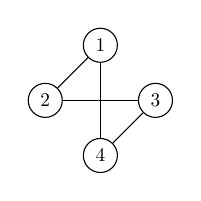
\begin{tikzpicture}[scale=.7, transform shape]
 		\node[style=circle,draw] (n1) at (1,2) {$1$};
 		\node[style=circle,draw] (n2) at (0,1) {$2$};
 		\node[style=circle,draw] (n3) at (2,1) {$3$};
 		\node[style=circle,draw] (n4) at (1,0) {$4$};
 		\draw (n1) edge (n2);
 		\draw (n1) edge (n4);
 		\draw (n3) edge (n2);
 		\draw (n3) edge (n4);
 		\end{tikzpicture}
 		\caption{A topology}
 		\label{fig:topequiv}
 	\end{subfigure}
    \begin{subfigure}[b]{0.6\textwidth}
    	\begin{tikzpicture}[scale=.8, transform shape]
    	\node [draw,outer sep=0,inner sep=3,minimum size=10] (n1) at (1,11) {$\begin{array}{l} 
    		1:(\{i\mapsto 1\},\epsilon),\\ 
    		2:(\{i\mapsto 2\},\langle{\it msg}\rangle),\\
    		3:(\{i\mapsto 1\},\epsilon),\\
    		4:(\{i\mapsto 0\},\epsilon),\end{array} %\begin{pmatrix}
    		%1 & 1 & 0 & 1 \\
    		%1& 1& 1 & 0 \\
    		%0 & 1  & 1 & 1 \\
    		%1 & 0 & 1 & 1
    		%\end{pmatrix}
    		$};
%    	\end{tikzpicture}
%    	\caption{Before applying counter abstraction}
%    	\label{fig::global}
%    \end{subfigure}
%    \begin{subfigure}[b]{0.3\textwidth}
%    	\begin{tikzpicture}[scale=.8, transform shape]
    	\node [draw,outer sep=0,inner sep=3,minimum size=10] (n2) at (7,11)
    	{$\begin{array}{l} ((\{i\mapsto 1\},\epsilon),\{1,3\}):\{1,3\},
    		\\((\{i\mapsto 2\},\langle{\it msg}\rangle),\{2,4\}):\{2\},\\
    		((\{i\mapsto 0\},\epsilon),\{2,4\}):\{4\}\end{array} $};
    	\draw[->, style=dashed] (n1) edge node[above]{reduced} (n2);
    	\end{tikzpicture}
    	\caption{Counter abstraction reduction}
    	\label{fig::reduction}
    \end{subfigure}    	
   \caption{Applying counter abstraction reduction with the assumed topology}
   \label{fig:counter-abstraction}
\end{figure*}


%To characterize the timing-dependent behavior of such protocols concerning mobility scenarios, Timed Rebeca was extended orthogonally with the topology concepts of wRebeca. For instance, the mobility scenario over which the maximal response time to find a routing path can be extracted via model checking technique. This was achieved by combining the floating-time idea of Timed Rebeca with network constraints exploited in wRebeca. 